\documentclass[twocolumn]{article}
\usepackage{graphicx} % Required for inserting images
\usepackage{newStyle}
\usepackage{titling}
\usepackage{stfloats}

\setlength{\droptitle}{-4em}

\title{StegoStamp Image Watermarking}
\author{Eugene Francisco}
\date{June 2026}

\begin{document}

\maketitle

\section{Overview}
Watermarking refers to the process of embedding information in generated data so as to label that data as having been generated by a model. This paper introduces StegoStamp, a novel way to watermark images, robust to common image transformations and lossy compression and virtually undetectable to the human eye. Inspired by Bui et al.\footnote{\TODO add reference}, we train a \textit{message encoder} to embed hidden bit sequences in the latent representation of images from a fixed autoencoder; alongside this, we train a \textit{secret decoder} to recover messages from possibly corrupted images. We use techniques from Tancik et al.\footnote{\TODO add reference} to make these watermarkers robust to spatial transformations like cropping and rotating, as well as regular image transformations like noising, blurring, and JPEG.

\section{Related Work}
Discuss Bui et al.\footnote{\TODO reference} and Tancik et al.\footnote{\TODO reference} and HiDDeN.

\section{Methods}
Watermarking derives from the much older process of steganography, where the goal is to conceal messages within another medium. Stated concretely, the goal of image watermarking is to take a so-called \textit{cover image} $c$ and message $m$ and generate a \textit{stego image} $\tilde c$ in which $m$ is somehow embedded; later on, a verifier should be able to take $\tilde c$ (possibly compressed or transformed in some way) and recover a message $\hat m$ which should be similar to $m$.

\begin{center}
	\begin{figure*}
	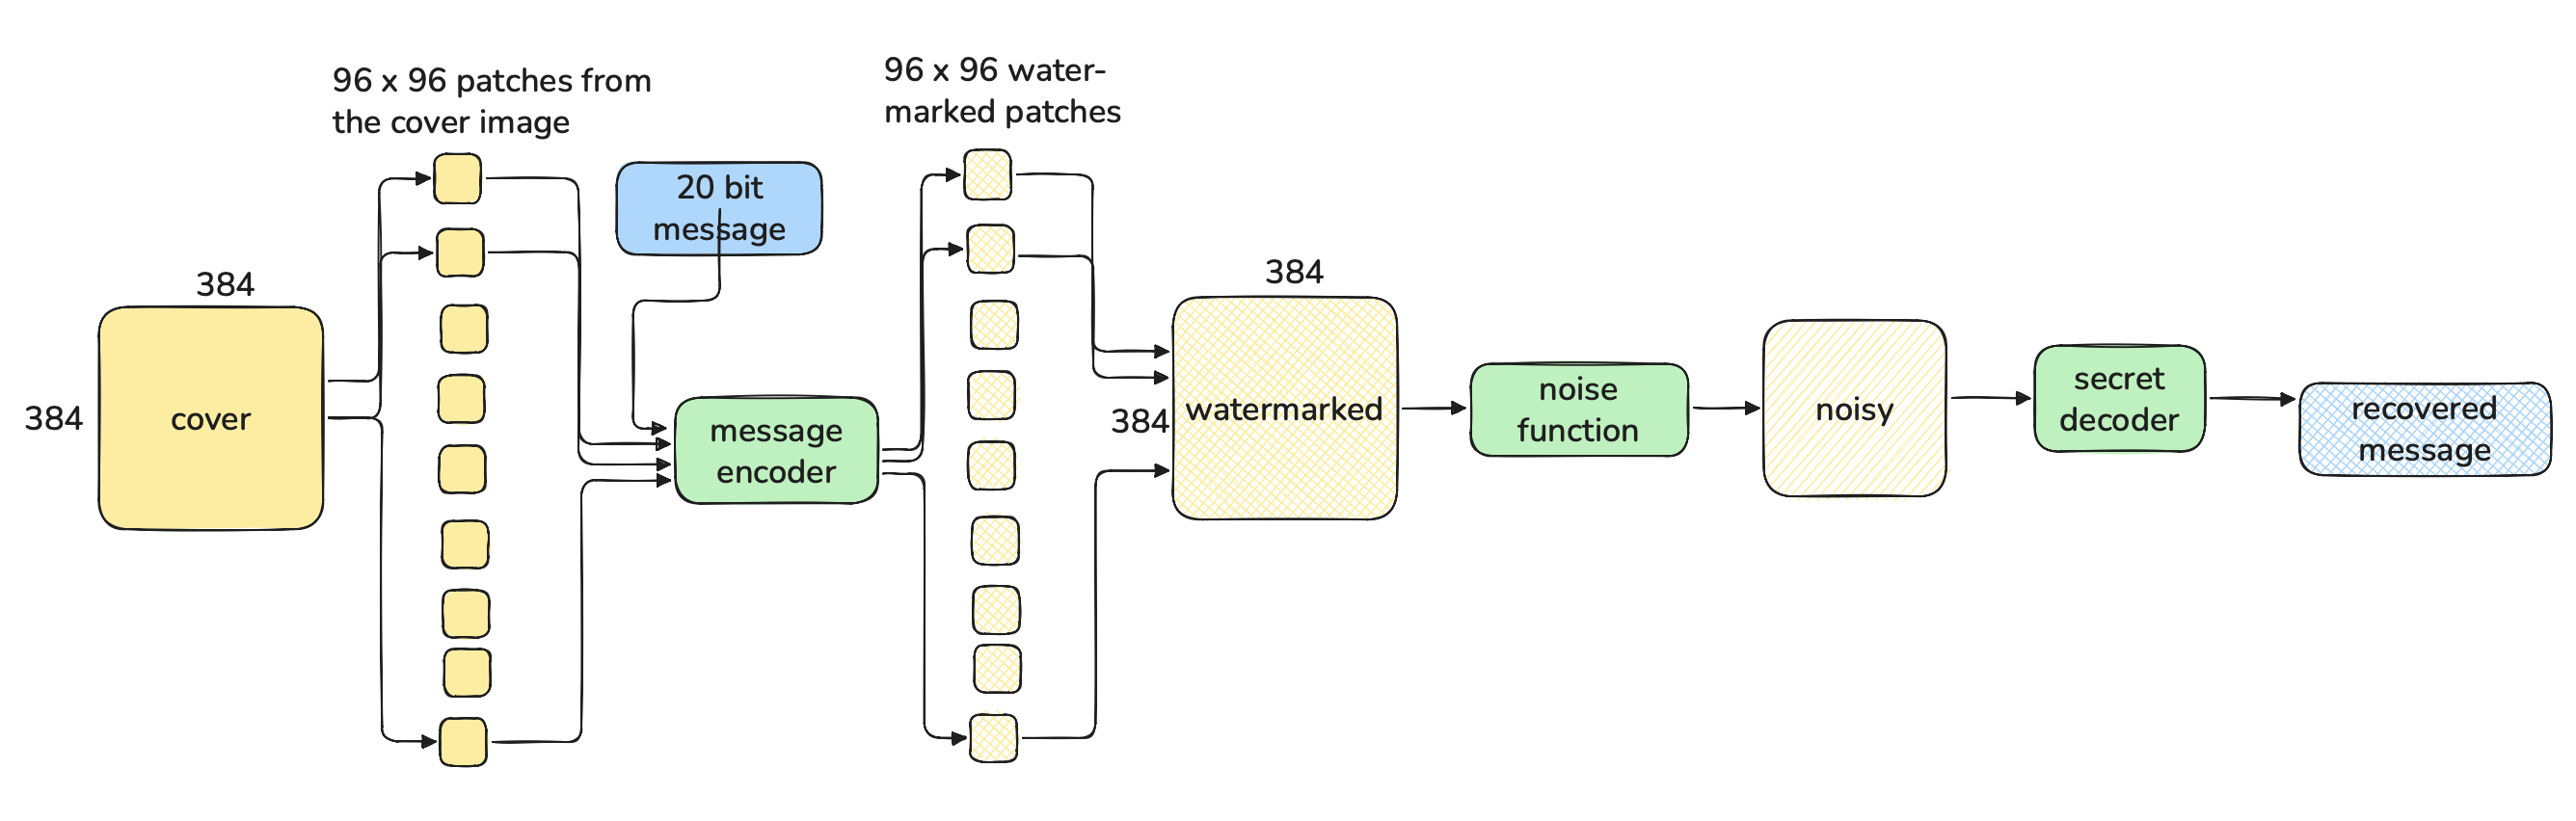
\includegraphics[scale=0.32]{images/architecture_plot.png}
	\caption{StegoStamp Watermarking and Decoding Architecture. The $\rm{message\ encoder}$ refers to $F_\theta$ and the $\rm{secret\ decoder}$ refers to $D_\varphi$.}
\end{figure*}

\end{center}
\subsection{Architecture}
StegoStamp trains two neural networks:
\begin{enumerate}[label=(\roman*)]
\item A message encoder $F_\theta$ which is used to encode messages and generate watermarked images.
\item A secret decoder $D_\varphi$ which is used to recover a message $\hat m$ from a (possibly corrupted) $\tilde c$.	
\end{enumerate}
These networks encode and decode in the following way:
\begin{enumerate}[label=(\roman*)]
\item Message Encoder: given a cover image $c$ of size $H\times W$ and a message $m$ of length $\ell$, we first partition $c$ into equal sized patches of size $P\times P$, where we assume $H, W$ are divisible by $P$. Let $\P$ be those patches. Fix an image autoencoder $(E, G)$, where $E$ is the encoder that sends images to the latent space and $G$ is a generator that creates images from latent variables.

For each patch $p\in \P$:
\begin{enumerate}[label=(\alph*)]
\item Create latent variable $z_p = E(g)$.
\item Create a latent offset $\delta = F_\theta(m)$.
\item Create a watermarked patch $\tilde p = G(z_p + \delta)$
\end{enumerate}
Stitch together the patches $\tilde p$ to get a watermarked image $\tilde c$ and return $\tilde c$.

The neural network $F_\theta$ is a very small convolutional neural network implemented in a similar way to Bui et al.
\item Secret Decoder: Given a (possibly corrupted) watermarked image $\tilde c$, the secret decoder returns $\hat m = D_\varphi(c)$. The neural network $D_\varphi(c)$ is implemented as a modified ResNet50 with the final flattening layer replaced by a $1\times 1$ CNN whose output is $\ell$ channeled. An average is taken across the width and height dimensions to retrieve an $\ell$ length vector of logits which are thresholded and returned as $\hat m$.

This last phase \textit{voting} step is taken from Zhu et al.'s HiDDeN.
\end{enumerate}
Here, $\theta$ and $\varphi$ are trainable parameters; note in particular that the autoencoder $(E, G)$ remain fixed and are not trained.
\subsection{Training Details}
We use the same training objectives as RoSteALS. $F_\theta$ is trained to minimize
\begin{align*}
	\L_{\mathrm{quality}} = \L_{\mathrm{LPIPS}}(\tilde c, c) + \alpha \Vert\gamma(c) - \gamma(\tilde c)\Vert_2^2\tag{1}
\end{align*}
where $\L_{\mathrm{LPIPS}}$ is the \textit{Learned Perceptual Image Patch Similarity} loss from Zhang et al.\footnote{\TODO Add reference} and $\gamma$ is a differentiable map from RGB to YUV color space. $\alpha$ is a hyperparameter to control objective weight. $D_\varphi$ is trained to minimize the binary cross entropy between $m$ and $\hat m$:
\begin{align*}
	\L_{\mathrm{recovery}} = \L_{\mathrm{BCE}}(m, \hat m).\tag{2}
\end{align*}
The combined training objective is then
\begin{align*}
	\L = \beta \L_{\mathrm{quality}} + \L_{\mathrm{recovery}}\tag{3}
\end{align*}
where $\beta$ is a weighting hyperparameter.




We use curriculum learning to train $F_\theta$ and $D_\varphi$. Learning is split into the following phases:
\begin{enumerate}
	\item Fix a single minibatch of images from the dataset. Train $F_\theta$ and $D_\varphi$ on this minibatch until bit accuracy of $m$ against $\hat m$ crosses $0.9$. Sample $m$'s bits uniformly and randomly. Before passing $\tilde c$ into $D_\varphi$, we choose with probability $1/2$ whether to crop $\tilde c$, in which case we crop $\tilde c$ to a random patch of fixed size (in our experiments, $3P\times 3P$).
	\item Expose $F_\theta$ and $D_\varphi$ to a much larger portion of the training set ($50{,}000$ images in our case). Train until bit accuracy reaches $0.8$ as this new exposure will likely drop the bit accuracy by a significant amount.
	\item Begin incrementing $\beta$ linearly by some amount $\delta_\beta$ until it reaches some $\beta_{\mathrm{max}}$, at which point continue training until bit accuracy reaches $0.95$.
	\item \TODO
	\item \TODO
\end{enumerate}

\section*{Implementation Details}
For simplicity, we trained on square images of size $384\times 384$ using a patch size of $P = 96$. \TODO how much are images cropped? All of our experiments are done with a message length of $\ell = 20$. We picked $\alpha = 1.5$ as in RoSteALS. We chose $\beta = 0.8$ (slightly lower than RoSteALS to account for more complicated decoding) and increment $\beta$ linearly until $\beta_{\mathrm{max}} = 10$ in training phase 3. We used the first $100{,}000$ images from the COCO training dataset from 2017. We optimize the objective in (3) using stochastic gradient descent (using PyTorch), a minibatch size of $8$, and the AdamW optimizer with a learning rate of $2\cdot 10^{-5}$.

We use a very small neural network for $F_\theta$ with only $9{,}168$ parameters. The network is described by the following PyTorch Sequential network: \TODO
\begin{verbatim}
nn.Linear(20, 12 * 12 * 3),
\end{verbatim}

\section{Experiments}
\TODO fill in with info about the experiments.

\section{Results}
\TODO fill in with photos of the images.

\begin{figure}
	\centering
	
\includegraphics[scale=0.25]{images/img1/cover.png}
	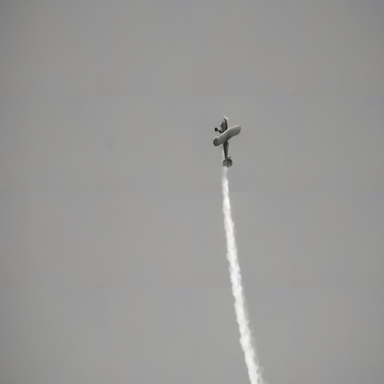
\includegraphics[scale=0.25]{images/img1/stego.png}\\
	
\includegraphics[scale=0.25]{images/img2/cover.png}
	
\includegraphics[scale=0.25]{images/img2/stego.png}\\
	
\includegraphics[scale=0.25]{images/img3/cover.png}
	
\includegraphics[scale=0.25]{images/img3/stego.png}\\
	
\includegraphics[scale=0.25]{images/img4/cover.png}
	
\includegraphics[scale=0.25]{images/img4/stego.png}\\
	
\includegraphics[scale=0.25]{images/img5/cover.png}
	
\includegraphics[scale=0.25]{images/img5/stego.png}
	\caption{Cover images (\textit{left}) and their watermarked counterparts (\textit{right}) produced by StegoPatch. Early experiments, light segmenting can still be seen in the airplane (top) and the pair talking (bottom).}
	\label{fig:stego_images}
\end{figure}


























\end{document}